% AASTeX v6.2
%\documentclass[preprint]{aastex62}

% ApJ Format
\documentclass[iop,revtex4,twocolumn,apj,numberedappendix,appendixfloats]{emulateapj}
\usepackage{apjfonts}
% Hyperlinks & Bookmarks
\usepackage[pagebackref=false,colorlinks=true,citecolor=blue,linkcolor=blue,breaklinks=true,bookmarks=true]{hyperref}
\usepackage{amsmath}
\usepackage{comment}

% Units
\newcommand{\kms}{km~s$^{-1}$}
\newcommand{\msun}{$M_{\odot}$}
\newcommand{\msunyr}{$M_{\odot}~{\rm yr}^{-1}$}
\newcommand{\lsun}{$L_{\odot}$}
\newcommand{\ergs}{erg~s$^{-1}$}
\newcommand{\cmsq}{cm$^{-2}$}
\newcommand{\um}{$\mu$m}
\newcommand{\uJy}{$\mu$Jy}
\newcommand{\sqdeg}{deg$^2$}
\newcommand{\lx}{$L_{\rm X}$}
\newcommand{\lmir}{$L_{\rm 12\mu m}$}
\newcommand{\loiii}{$L_{\rm [OIII]}$}
% Emission lines
\newcommand{\Ha}{H$\alpha$}
\newcommand{\Hb}{H$\beta$}
\newcommand{\OII}{[O\,{\sc ii}]}
\newcommand{\OIIlam}{[O\,{\sc ii}]\,$\lambda$3727}
\newcommand{\SII}{[S\,{\sc ii}]}
\newcommand{\OIII}{[O\,{\sc iii}]}
\newcommand{\OIIIlam}{[O\,{\sc iii}]\,$\lambda$5007}
\newcommand{\NII}{[N\,{\sc ii}]}
\newcommand{\NeIII}{[Ne\,{\sc iii}]}
% special 
\newcommand{\nod}{\nodata}

\newcommand{\angstrom}{\mbox{\normalfont\AA}}
\newcommand{\reff}{$R_{\rm eff}$}
\newcommand{\ewha}{EW(H$\alpha$)}
\newcommand{\logm}{log({\it M}/M$_{\odot}$)}
%\newcommand{\arcsec}{\prime\prime}

% citations
\defcitealias{Fu18}{Paper I} 

\usepackage{epstopdf}

\begin{document}

\title{SDSS-IV MaNGA: Radial Profiles of Specific Star Formation Rate in Nearby Interacting Galaxies}

\author{
Joshua L. Steffen\altaffilmark{1}, 
Hai Fu\altaffilmark{1}, and 
MaNGA Team 
}
\altaffiltext{1}{Department of Physics \& Astronomy, The University of Iowa, 203 Van Allen Hall, Iowa City, IA 52242}

\begin{abstract}

\end{abstract}

\keywords{galaxies: active --- galaxies: nuclei --- galaxies: interactions}

%%%%%%%%%%%%%%%%%%%%%%%%%%%%%%%%%%%%%%%%%%%%%%%%%%%%
\section{Introduction}\label{sec:intro}

%%%Galaxy Evolution%%%
%{\it In $\Lambda$CDM, galaxy evolution is a hierarchical, bottom-up process. Galaxies are created in a process where large dark matter halos are formed out of the merging of smaller dark matter pockets and galaxies form within the dark matter halos \citep{White:1978}. The subsequent merging of dark matter halos leads to a scenario where a large central galaxy is surrounded by a cluster of smaller satellite galaxies within a single dark matter halo. The satellite galaxies lose kinetic energy through dynamical friction \citep{Chandrasekhar:1943} and will eventually merge with the central galaxy. The dynamical timescale for a merger event is on the order of 1 Gyr, which means that present day galaxies could have undergone multiple merger events during their lifetimes.

%This means that the massive galaxies in the universe today are the product of the merging of several smaller galaxies. In fact, cosmological hydrodynamical simulations have shown that repeated merger events may be responsible for as much as $\sim$60\% of stellar mass in massive galaxies like M87 (e.g. \citet{Rodriguez-Gomez:2016}; \citet{Pillepich:2018}). 

%This bottom-up process is still ongoing and can be seen in the Local Group with the Milky Way's collection of satellite galaxies. The Milky Way has an ongoing minor merger with its closest companion, the Canis Major dwarf galaxy \citep{Martin:2004} and is on track to merge with the Andromeda galaxy. }\\

%%%%%
In the $\Lambda$CDM model, galaxy evolution is a hierarchical process. Over the lifetime of the universe, smaller galaxies have iteratively merged with each other to form more massive galaxies. In fact, cosmological hydrodynamical simulations have shown that repeated merger events may be responsible for as much as $\sim$60\% of stellar mass in massive galaxies like M87 (e.g. \citet{Rodriguez-Gomez:2016}; \citet{Pillepich:2018}). \\
%%%%%

%%%Simulations%%%
%{\it Interacting galaxies were originally known as peculiar galaxies, named for their unusual shapes and morphologies. These peculiar galaxies were often seen to have nearby, neighboring galaxies and, because of this, it was suspected that the unusual features such as tails, bridges, or warped disks were the product of the gravitational tidal forces between the galaxies \citep{Zwicky:1959}. 

%\citet{Toomre:1972} investigated the idea using N-body simulations to model galaxy interactions. They used concentric rings of stars which were gravitationally bound to a central, massive nucleus. In their work, \citet{Toomre:1972} were able to demonstrate how the tidal tails found in peculiar galaxies could be the result of galaxy interactions. This confirmed the idea that peculiar galaxies are the result of galaxies interactions. 

%Since the N-body simulations from \citet{Toomre:1972}, more advanced simulations have been made which model the gas-dynamics within the interacting galaxies. These N-body plus gas-dynamics simulations showed how the tidal torques acting on the galaxy disks cause the formation of barred structures \citep{Barnes:1991}. As the bars are formed, the gases within the disk lose their angular momentum and get funneled into the center of the galaxy. The inflowing gases impact upon the gases already present in the galactic center and trigger a burst of new star formation \citep{Barnes:1996, Mihos:1996}. 

%The inflows bring in metal-poor gases from the disk, diluting the nuclear metal content of galaxy's center \citep{Rupke:2010, Perez:2011, Scudder:2012}. The inflows can also trigger supermassive black hole (SMBH) accretion \citep{Capelo:2017}.

%Another common feature of peculiar galaxies is that they tend to have much bluer B$-$V color than other galaxy types \citep{Larson:1978}. The galaxies within the "Blue Cloud" on the color-magnitude diagram (CMD) are often associated with having active star formation. \citet{Larson:1978} identified that the galaxies showing deviations in color from normal galaxies are the galaxies which displayed features like tidal tails. This indicated that the violent disturbances subjected to interacting galaxies could trigger a large burst of star formation.} \\

%%%%%
The internal dynamics of these interacting galaxies were first modeled in the seminal work, \citet{Toomre:1972}. Since then, hydrodynamical simulations have expanded upon the N-body simulations of \citet{Toomre:1972} by modeling gas-dynamics within the galaxies. These simulations show how barred structures develop within the disks of the interacting galaxies due to the tidal torques between them \citep{Barnes:1991}. As the bars form, the gases within the galaxy's disk lose angular momentum and get funneled into the centers of the galaxies. 

When the gas-inflows impact upon the gases in the nucleus of galaxy a burst of new star formation in triggered \citep{Barnes:1996, Mihos:1996}. These gas inflows will also bring metal-poor gases from the disk into the center of the galaxy which can dilute the central metallicity \citep{Rupke:2010, Perez:2011, Scudder:2012}. The gas-inflows may also be able to make it into very center of the galaxy and trigger supermassive black hole (SMBH) accretion \citep{Capelo:2017}. \\
%%%%%

%%%Observations%%%
%{\it Interacting galaxies have been studied extensively with large spectroscopic surveys. It has been shown that interacting galaxies feature higher levels of star formation than isolated galaxies in the surveys; CfA2  \citep{Barton:2000, Woods:2006}, 2dF \citep{Lambas:2003}, AEGIS \citep{Lin:2007}, SDSS \citep{Ellison:2008}, COSMOS \citep{Kartaltepe:2007,Xu:2012}, PRIMUS \citep{Wong:2011}, and GAMA \citep{Robotham:2014}.

%The levels of star formation enhancement was shown to increase with closer projected separations \citep{Ellison:2008, Scudder:2012, Patton:2013}. These works indicate that the merger event ignites a burst of star formation after the passage of the first pericenter and that the burst of star formations begins to fade as the galaxies separate. \citet{Patton:2013} showed that this burst of star formation lingers as far out as projected separations of 150 kpc. The level of enhancement is also tied to the mass ratio, $|\Delta {\rm log}\,M|$, between the galaxies where major mergers, $\left( | \Delta {\rm log}\,M | \le 0.6\right)$, have larger rates of enhancement in comparison to minor mergers, $\left(0.6 < |\Delta {\rm log}\,M| \le 1.0\right)$ \citep{Ellison:2008}. 

%These single-fiber spectroscopic studies have been also used to study the nuclear metal content of the galaxy pairs. The galaxy pairs show weak levels of metallicity dilution in their centers, $\Delta$log(O/H) $\sim -0.05$ dex \citep{Ellison:2008, Scudder:2012}. The central metallicity dilution helps confirm the idea that the merger induced star formation is triggered by gas flows from the metal-poor galactic disks.} \\

%%%%%
Centrally enhanced star formation has also been observed in large spectroscopic surveys including; CfA2  \citep{Barton:2000, Woods:2006}, 2dF \citep{Lambas:2003}, AEGIS \citep{Lin:2007}, SDSS \citep{Ellison:2008}, COSMOS \citep{Kartaltepe:2007,Xu:2012}, PRIMUS \citep{Wong:2011}, and GAMA \citep{Robotham:2014}.

This star formation enhancement increases with closer projected separations between the two galaxies \citep{Ellison:2008, Scudder:2012} but has still shown to be detectable at wide projected separations of 150 kpc \citep{Patton:2013}. The level of the star formation enhancement also increases with smaller stellar mass ratios, $|\Delta log {\it M} |$, between the two galaxies \citep{Ellison:2008}. \\
%%%%%

%%%Integral Field Spectroscopy%%%
%{\it The advent of large integral field spectroscopic (IFS) surveys has opened a new door in studying nearby galaxies. Previous single-fiber spectroscopic studies limit the degree to which we can study galaxy parameters like star formation or metallicity since these surveys are limited to covering only the centers of galaxies. IFS surveys allocate an entire bundle of fiber-optic cables, called integral field units (IFUs), to individual galaxies, giving us spectroscopy across the whole disk of the galaxies. The current set of IFS surveys include the Calar Alto Legacy Integral Field Area (CALIFA) survey which is based in Spain and covered $\sim$600 galaxies \citep{Sanchez:2012}, the Sydney-AOO Multi-object Integral field spectrograph (SAMI) survey which is based in Australia which plans to cover 3000 galaxies \citep{Croom:2012}, and the Mapping Nearby Galaxies at Apache Point Observatory (MaNGA) survey which is based in New Mexico and plans to cover 10,000 galaxies \citep{Bundy:2015}. In this work we will be using the MaNGA survey since it is the largest IFS survey to date.

%Because of these new IFS surveys, parameters like star formation and gas-phase metallicity can be studied spatially in detail. These IFS surveys have also been used to study the distribution of star formation in interacting galaxies. \citet{Barrera-Ballesteros:2015} utilized the spatial resolution of the CALIFA survey in galaxy pairs by varying the aperture sizes from which SFR is extracted from. They found that the SFR is enhanced in the centers of galaxy pairs by a factor of 2$-$3$\times$ and that SFR is moderately suppressed by $\sim$0.74$\times$ in their disks. \citet{Barrera-Ballesteros:2015} also found that, in contrast to previous single fiber studies, that the metallicity found in the centers of galaxy pairs are not significantly different from their controls. 

%\citet{Pan:2019} used the MaNGA survey to study the radial profiles of specific star-formation rate (sSFR; where sSFR is the SFR of a region divided by the stellar mass of the region) in interacting galaxies. The galaxy pairs featured strong central enhancement of sSFR ($\sim$0.35 dex), but also weak enhancement of sSFR in their disks ($\sim$0.1$-$0.2 dex). \citet{Pan:2019} also studied the sSFR profiles across different merger stages. Galaxies pairs only showed signs of sSFR enhancement after the first pericenter, i.e. only pairs with visual morphological disturbances showed sSFR enhancement.

%The MaNGA survey has also been used to study the radial profiles of post merger galaxies (galaxy mergers which have coalesced but still show some tidal features). The post mergers featured a central enhancement to SFR surface density of $\sim$ 2.5$\times$ and show a weak metallicity dilution of $\sim$$-$0.04 dex across their disks \citep{Thorp:2019}. } \\

%%%%%
With the recent large integral field spectroscopic (IFS) surveys, interacting galaxies can be studied in unprecedented spatial detail. Where previous spectroscopic surveys where limited to the nucleus of the interacting galaxies, the new IFS surveys will be able to study both the nuclei and the disks of the interacting galaxies. 

\citet{Barrera-Ballesteros:2015} studied star formation in interacting galaxies with the CALIFA\footnote{Calar Alto Legacy Integral Field Area} survey using variable aperture sizes from which the star formation rate (SFR) is extracted from. \\
%%%%%

%%%Purpose%%%
%{\it In our previous work, \citet{Fu:2018}, we built a sample of galaxies pairs where both galaxies were found within the field of view of a single MaNGA IFU. We confirmed the theoretical expectation that the MaNGA pair fraction will increase with higher stellar masses and wider physical spatial coverage. We found that $\sim$5.7\% of the MaNGA galaxies have close spectroscopic companions. In \citet{Fu:2018} we further analyzed the presence of AGN in galaxy pairs and found that AGN duty cycle is preserved in individual galaxies; however, the population of binary AGN is increased. 

%In this work we will expand upon our pair sample from \citet{Fu:2018} with the most recent MaNGA Data Release, DR16, and supplement the sample with MaNGA galaxies which have companions identified outside of their IFUs. The galaxy pairs within the fields of view of a single IFU will allow us to study the closest galaxy pairs while the expanded sample of galaxy pairs identified outside of the MaNGA IFUs will allow us to expand the separation coverage of the sample. 

%With the expanded pair sample, we will study radial profile of star formation in the galaxy pairs. First we will address whether or not galaxy pairs experience enhanced star formation from the merger event. Second, we will study if the star formation enhancement is confined to the centers of the paired galaxies or if the enhancement extends into their disks. Afterwords, we will address how other parameters pertaining to the galaxy pairs can affect the merger induced star formation. 

%\begin{enumerate}

%\item Does the total stellar mass of a galaxy affect the level of enhancement to the specific star-formation rate? That is to say, are low mass galaxies enhanced at the same level as high mass galaxies?

%\item Does the stellar mass ratio between the interacting galaxy and its companion affect the rate of enhancement to the specific star-formation rate? We will see if galaxy mergers with roughly the same stellar mass are more efficient at inducing star-formation in comparison to massive galaxies absorbing dwarf galaxies. 

%\item Does the projected separation between the companion galaxies affect the rate of enhancement to the specific star-formation rate. We would expect the companions with the closest separations to have the highest rate of enhancement since they are the most likely to have recently undergone their first pericenter. We can also see how separated a set of companions can be and still show enhancement to their star-formation. 

%\item Does the merger induced star formation contribute a significant amount of new stellar mass growth to the galaxies?

%\end{enumerate}

%By answering these questions we hope to gain insight on the relevance of individual galaxy merger events in the context of galaxy evolution at low redshift. }\\

% Organization
This paper is organized as follows; in Section \ref{sec:data} we will discuss the detail of the MaNGA survey, in Section \ref{sec:analysis} we will discuss how we extract emission lines from the MaNGA survey and how we calculate the star formation from them, in Section \ref{sec:pair} we discuss the construction of our pair sample, in Section \ref{sec:control} we discuss the construction of our control sample, in Section \ref{sec:radial} we build the radial profiles for the pair and control galaxies, in Section \ref{sec:results} we discuss the results of the survey, in Section \ref{sec:discussion} we discuss our results in the context of other surveys, and in Section \ref{sec:sum} we summarize and conclude the work. 

%%%%%%%%%%%%%%%%%%%%%%%%%%%%%%%%%%%%%%%%%%%%%%%%%%%%
\section{Data}\label{sec:data}


%%%%%%%%%%%%%%%%%%%%%%%%%%%%%%%%%%%%%%%%%%%%%%%%%%%%
\section{Emission Lines}\label{sec:analysis}


%%%%%%%%%%%%%%%%%%%%%%%%%%%%%%%%%%%%%%%%%%%%%%%%%%%%
\section{Pair Sample}\label{sec:pair}


%%%%%%%%%%%%%%%%%%%%%%%%%%%%%%%%%%%%%%%%%%%%%%%%%%%%
\section{Control Sample}\label{sec:control}


%%%%%%%%%%%%%%%%%%%%%%%%%%%%%%%%%%%%%%%%%%%%%%%%%%%%
\section{Radial Profiles}\label{sec:radial}


%%%%%%%%%%%%%%%%%%%%%%%%%%%%%%%%%%%%%%%%%%%%%%%%%%%%
\section{Results}\label{sec:results}


%%%%%%%%%%%%%%%%%%%%%%%%%%%%%%%%%%%%%%%%%%%%%%%%%%%%
\section{Discussion}\label{sec:discussion}


%%%%%%%%%%%%%%%%%%%%%%%%%%%%%%%%%%%%%%%%%%%%%%%%%%%%
\section{Summary and Conclusion}\label{sec:sum}






\acknowledgments

% funding
J.S. and H.F. acknowledge support from the National Science Foundation (NSF) grant AST-1614326 and University of Iowa funds. 

%%%%%%%%%%%%%%%%%%%% REFERENCES %%%%%%%%%%%%%%%%%%
\bibliographystyle{aasjournal}
\bibliography{mergerbib}

%%%%%%%%%%%%
% Appendix
%%%%%%%%%%%%

\hbox{}\clearpage

\appendix

\section{Figures}

%%%%%%%%%%%%%%%%%%%%%%%%%%%%%%%%%%%%%%%%%%%%%%
\begin{figure}
\centering
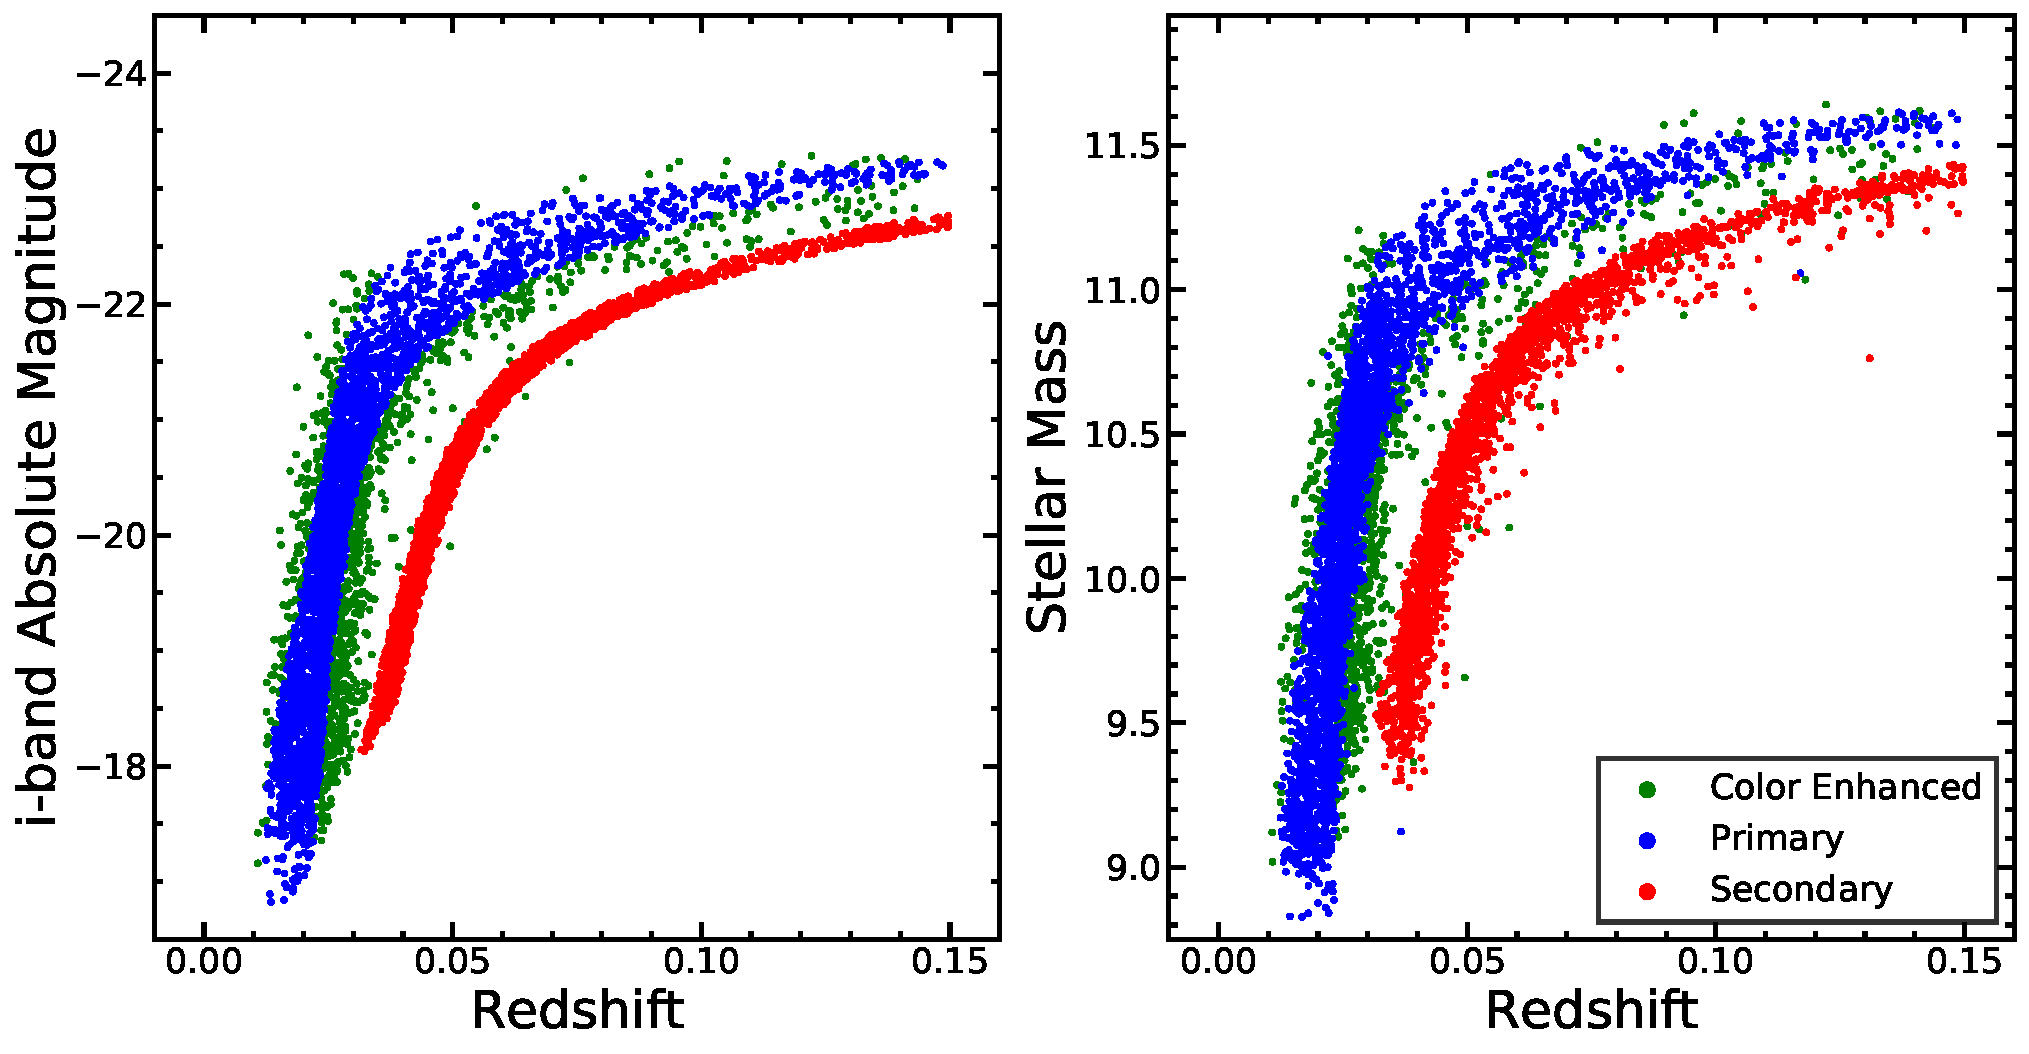
\includegraphics[width=\linewidth]{fig/Mi-z.pdf}
\caption[The luminosity - redshift distribution and mass - redshift distribution of the MaNGA sample.]{On the left is the luminosity - redshift distribution of the MaNGA sample. The figure illustrates the unique distribution of the MaNGA sample. On the right, I replace the luminosity with stellar mass from the NSA catalog.}
\label{fig:Mi_z}
\end{figure}
%%%%%%%%%%%%%%%%%%%%%%%%%%%%%%%%%%%%%%%%%%%%%%

%%%%%%%%%%%%%%%%%%%%%%%%%%%%%%%%%%%%%%%%%%%%%%
\begin{figure}
\centering
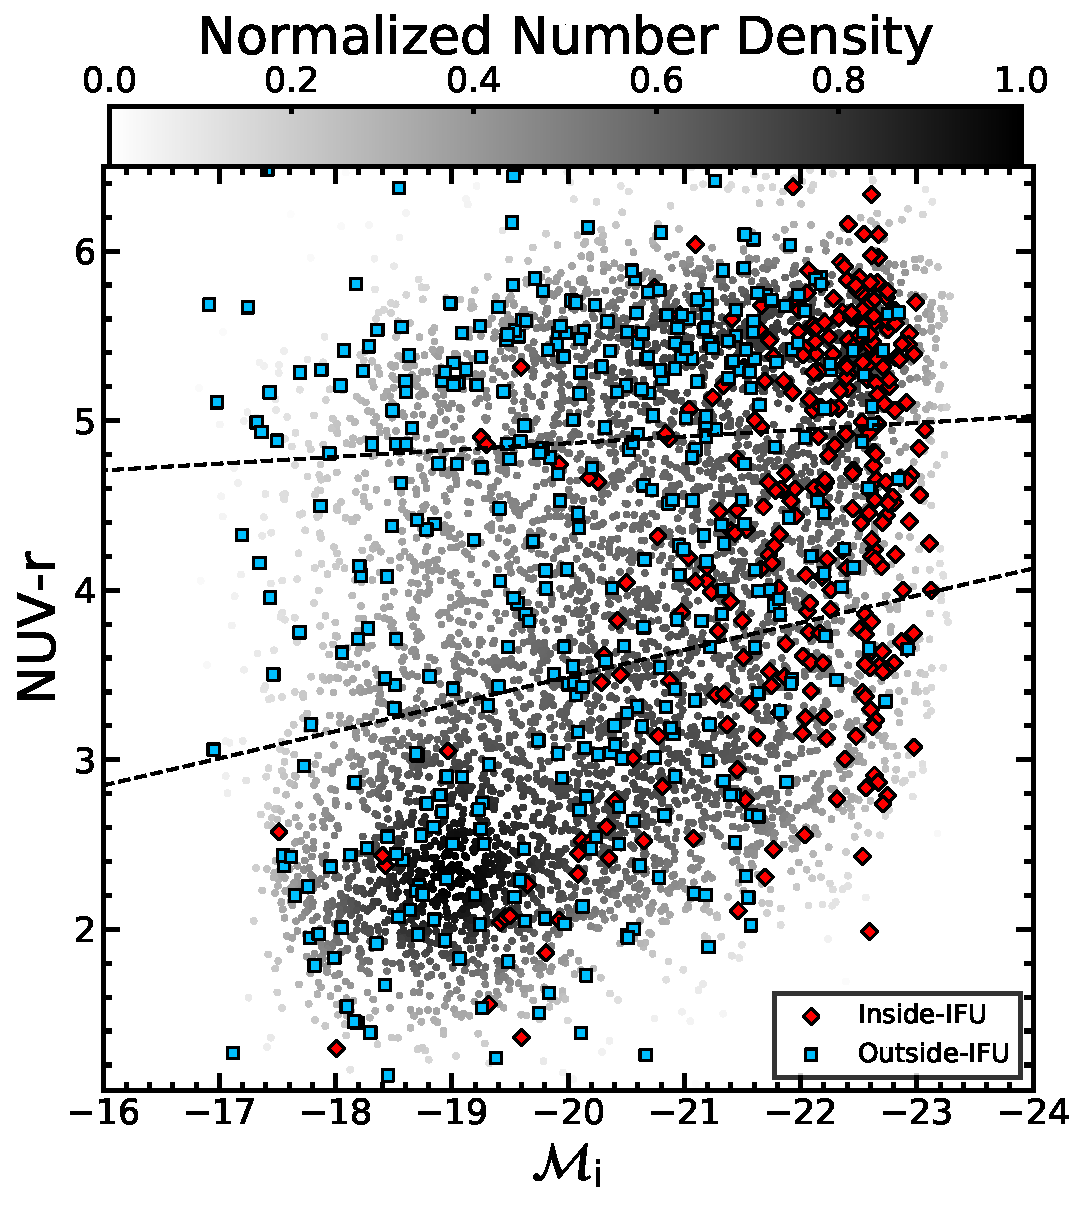
\includegraphics[width=3in]{fig/color-mag.pdf}
\caption[Color-magnitude distribution of the MaNGA galaxies]{Color-magnitude diagram for MaNGA galaxies ({\it colored circles}). The color of the symbol reflects the local density around each data point in this color-magnitude plane, as indicated by the color bar on the top. The MaNGA galaxies with close companions are marked with {\it grey diamonds}. From top to bottom, the dashed lines divide the sample into red sequence, green valley, and blue cloud. The star-forming galaxy sample used in this paper are the galaxies below the lower dividing line.}
\label{fig:CMD}
\end{figure}
%%%%%%%%%%%%%%%%%%%%%%%%%%%%%%%%%%%%%%%%%%%%%%

%%%%%%%%%%%%%%%%%%%%%%%%%%%%%%%%%%%%%%%%%%%%%%
\begin{figure}
\centering
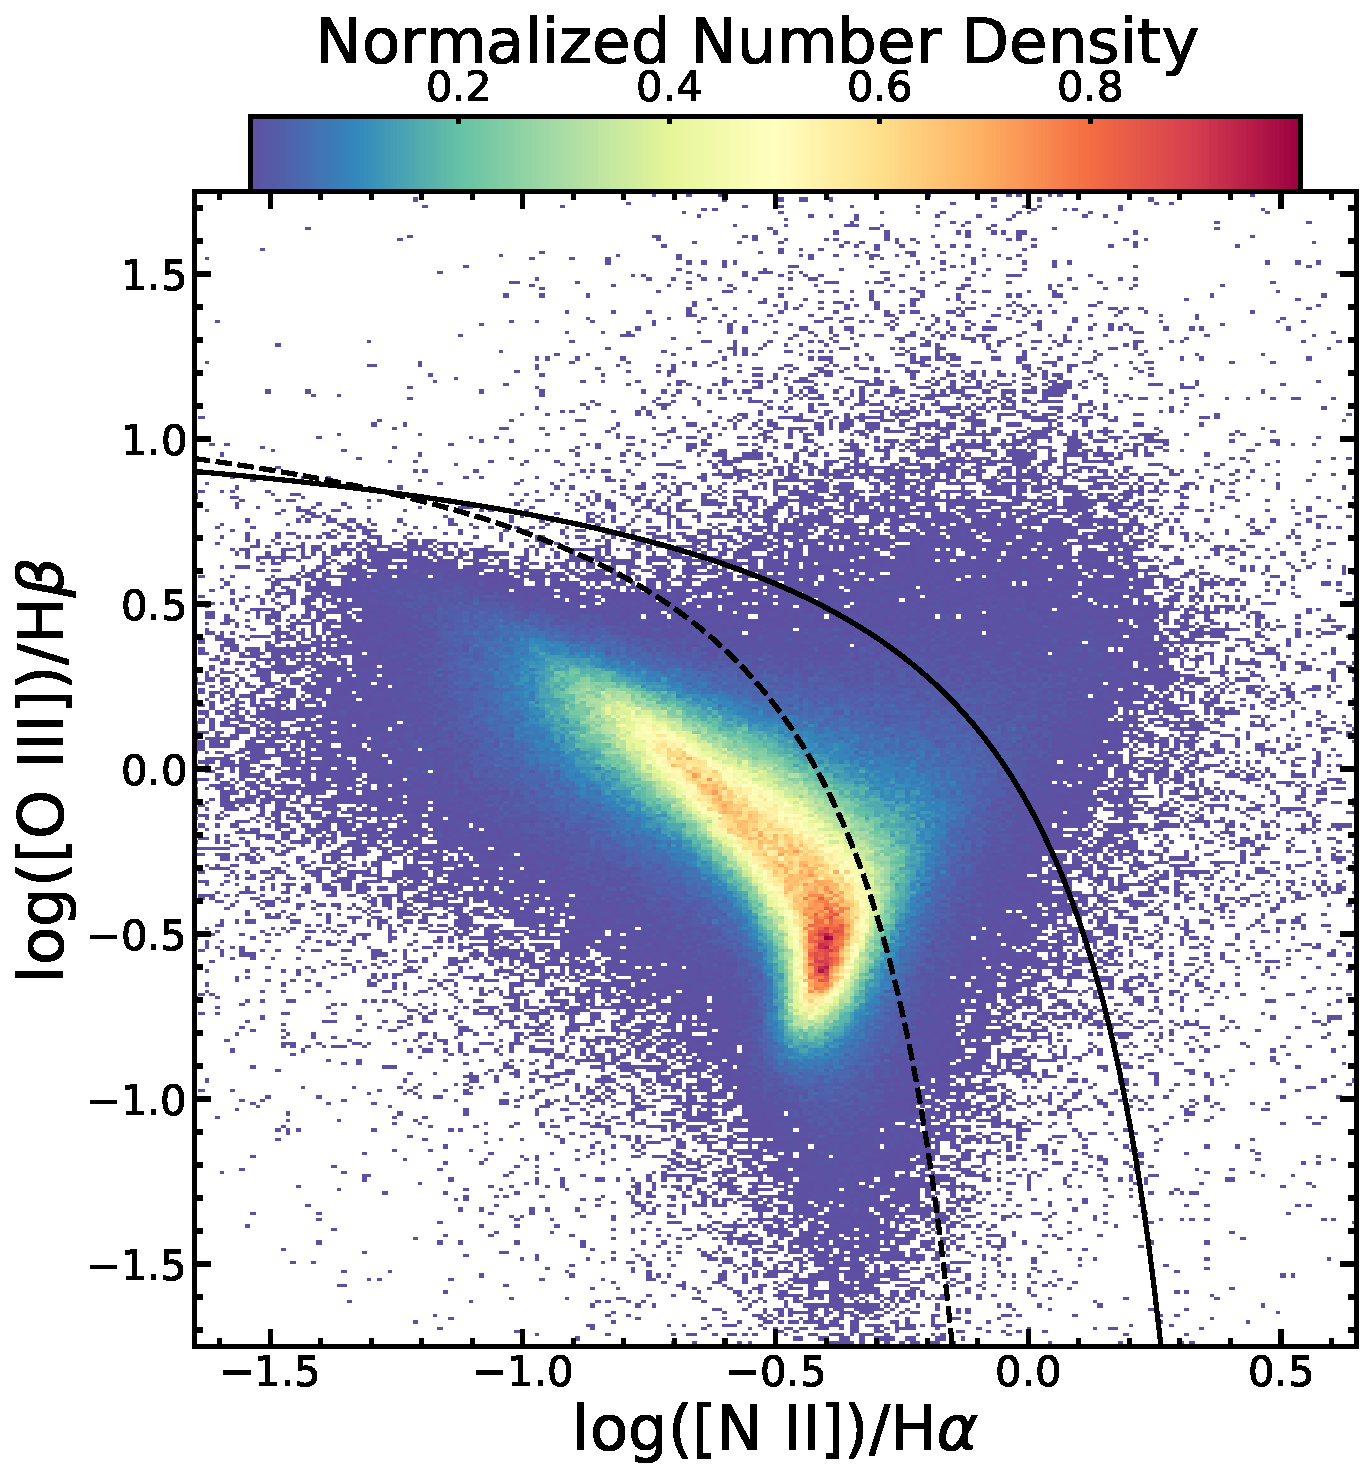
\includegraphics[width=3in]{fig/bpt_spax.pdf}
\caption[BPT classification of MaNGA spaxels.]{The 2-D histogram showing the BPT classification \citep{Baldwin:1981} of individual spaxels within our star-forming control and pair samples. The color of each bin represents the number density of spaxels, normalized to one. The black line represents the theoretically determined maximum starburst line of \citet{Kewley:2001}. This shows the capability of the CMD to select star-forming galaxies as most of the spaxels within the selected galaxies fall beneath the starburst line.}
\label{fig:bpt_spax}
\end{figure}
%%%%%%%%%%%%%%%%%%%%%%%%%%%%%%%%%%%%%%%%%%%%%%

%%%%%%%%%%%%%%%%%%%%%%%%%%%%%%%%%%%%%%%%%%%%%%
\begin{figure}
\centering
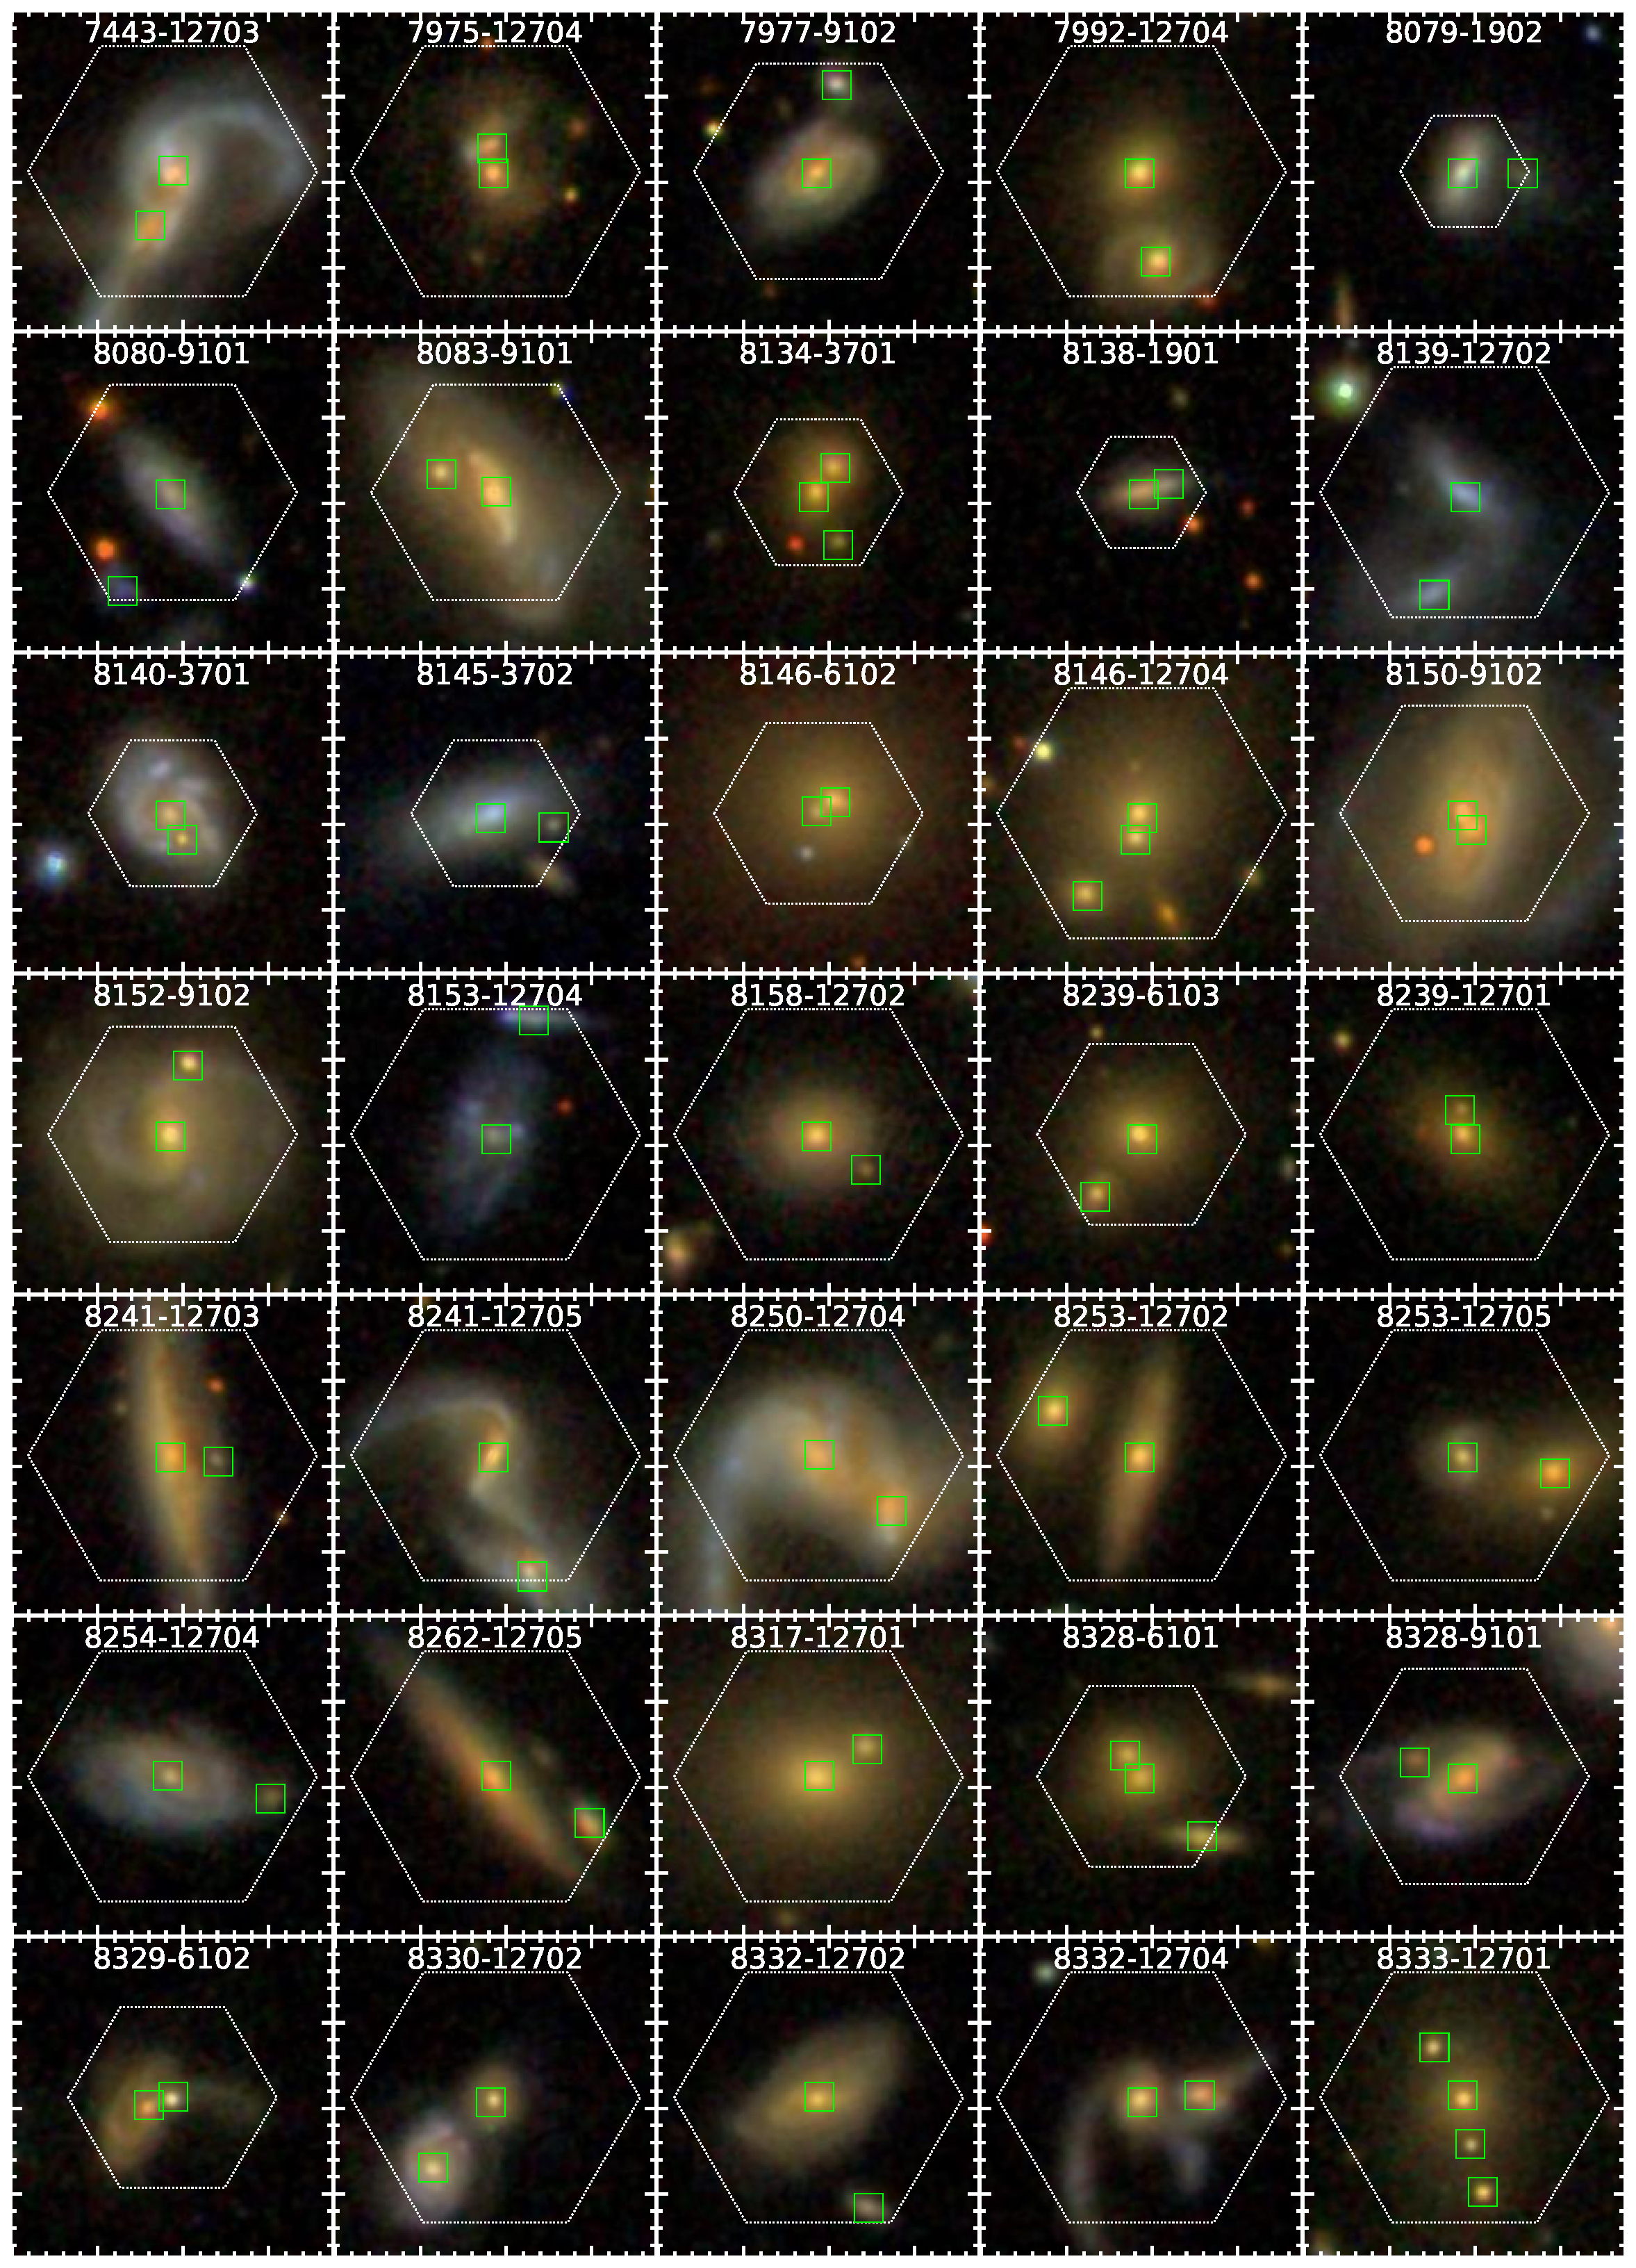
\includegraphics[width=\linewidth]{fig/pair_collage.pdf}
\caption[A collage of a subset of the inside-IFU pairs.]{A collage of a subset of the inside-IFU pairs. Each panel contains a 40$^{\arcsec}$ cutout of the SDSS pseudocolor image for the galaxy pair. The minor ticks on each panel's axis represents 2$^{\arcsec}$. The green squares highlight the identified galaxy pairs. }
\label{fig:collage}
\end{figure}
%%%%%%%%%%%%%%%%%%%%%%%%%%%%%%%%%%%%%%%%%%%%%%

%%%%%%%%%%%%%%%%%%%%%%%%%%%%%%%%%%%%%%%%%%%%%%
\begin{figure*}
\centering
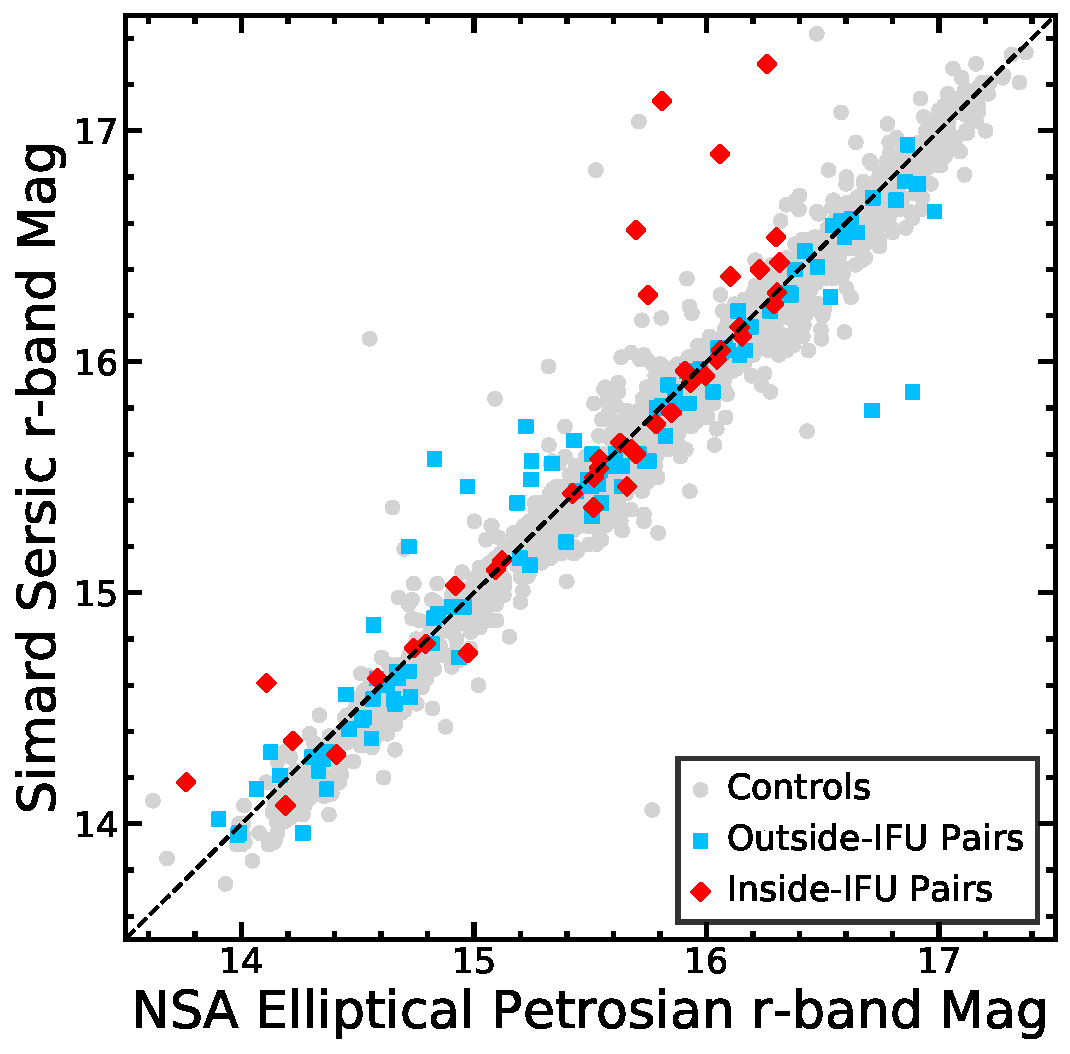
\includegraphics[width=3in]{fig/mag_comp.pdf}
\caption[The comparison between the r-band magnitudes in Simard+11 and NSA catalog]{The comparison between the S\'ersic r-band apparent magnitude in \citet{Simard:2011} and the Elliptical Petrosian r-band apparent magnitude. The grey circles represent galaxies in the control sample, the blue squares represent galaxies in the outside-IFU sample, and the red diamonds represent the galaxies in the inside-IFU sample. Regardless of the sample, all of the galaxies covered by both of the catalogs have a similar apparent magnitude calculated from either sample.}
\label{fig:mag_comp}
\end{figure*}
%%%%%%%%%%%%%%%%%%%%%%%%%%%%%%%%%%%%%%%%%%%%%%

%%%%%%%%%%%%%%%%%%%%%%%%%%%%%%%%%%%%%%%%%%%%%%
\begin{figure*}
\centering
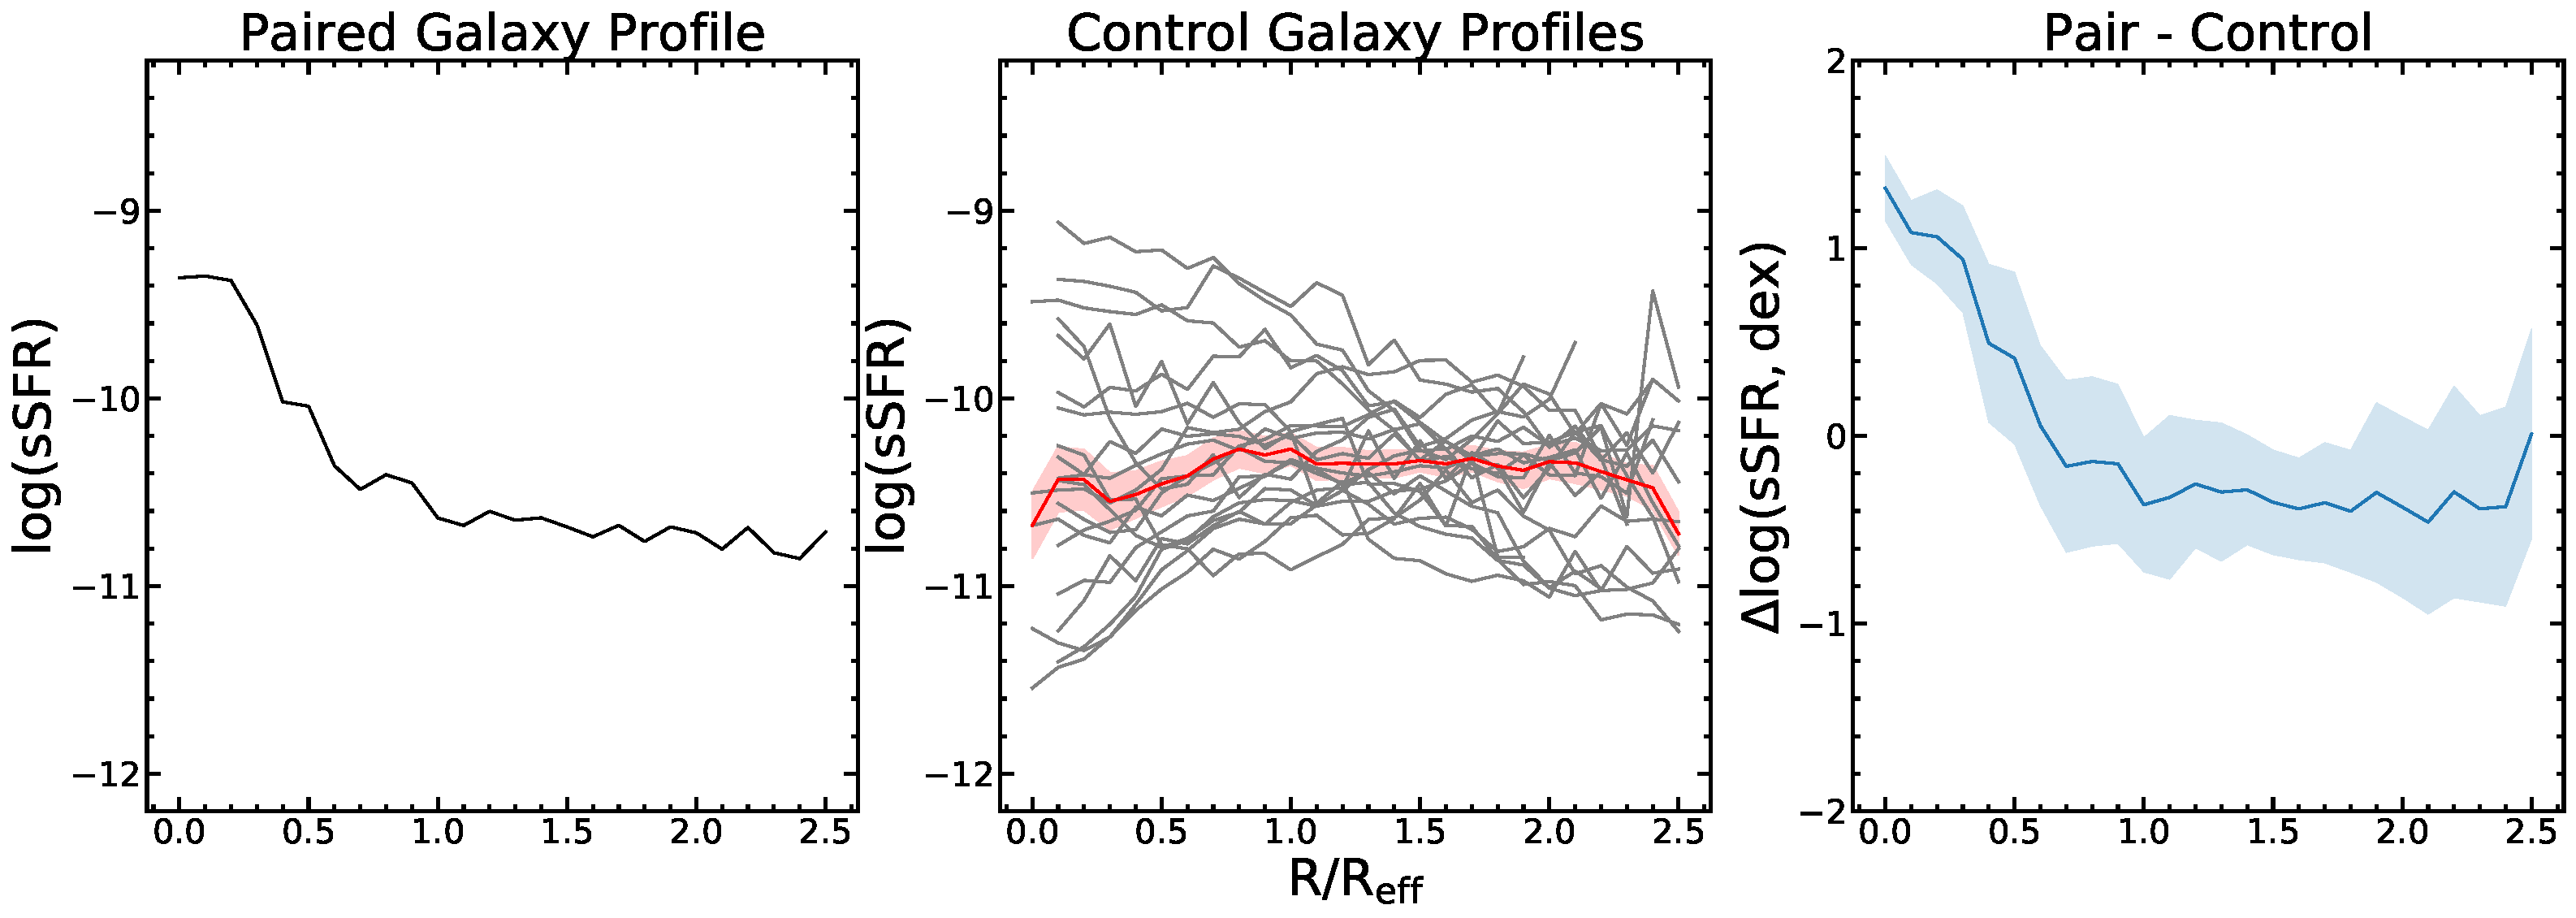
\includegraphics[width=\linewidth]{fig/8083-12703.pdf}
\caption[Example of the difference profiles for the mass-redshift selected control sample.]{The process for building the tailored control sample. The Left panel shows the paired galaxy's profile for sSFR. The Middle panel shows the profiles for sSFR for the selected 20 control galaxies in gray. The red profile is the median profile of the 20 control galaxies where the highlighted region about the profile is the standard error of the mean. The Right panel shows the difference between pair's profile and the stacked control profile.}
\label{fig:dex}
\end{figure*}
%%%%%%%%%%%%%%%%%%%%%%%%%%%%%%%%%%%%%%%%%%%%%%

%%%%%%%%%%%%%%%%%%%%%%%%%%%%%%%%%%%%%%%%%%%%%%
\begin{figure*}
\centering
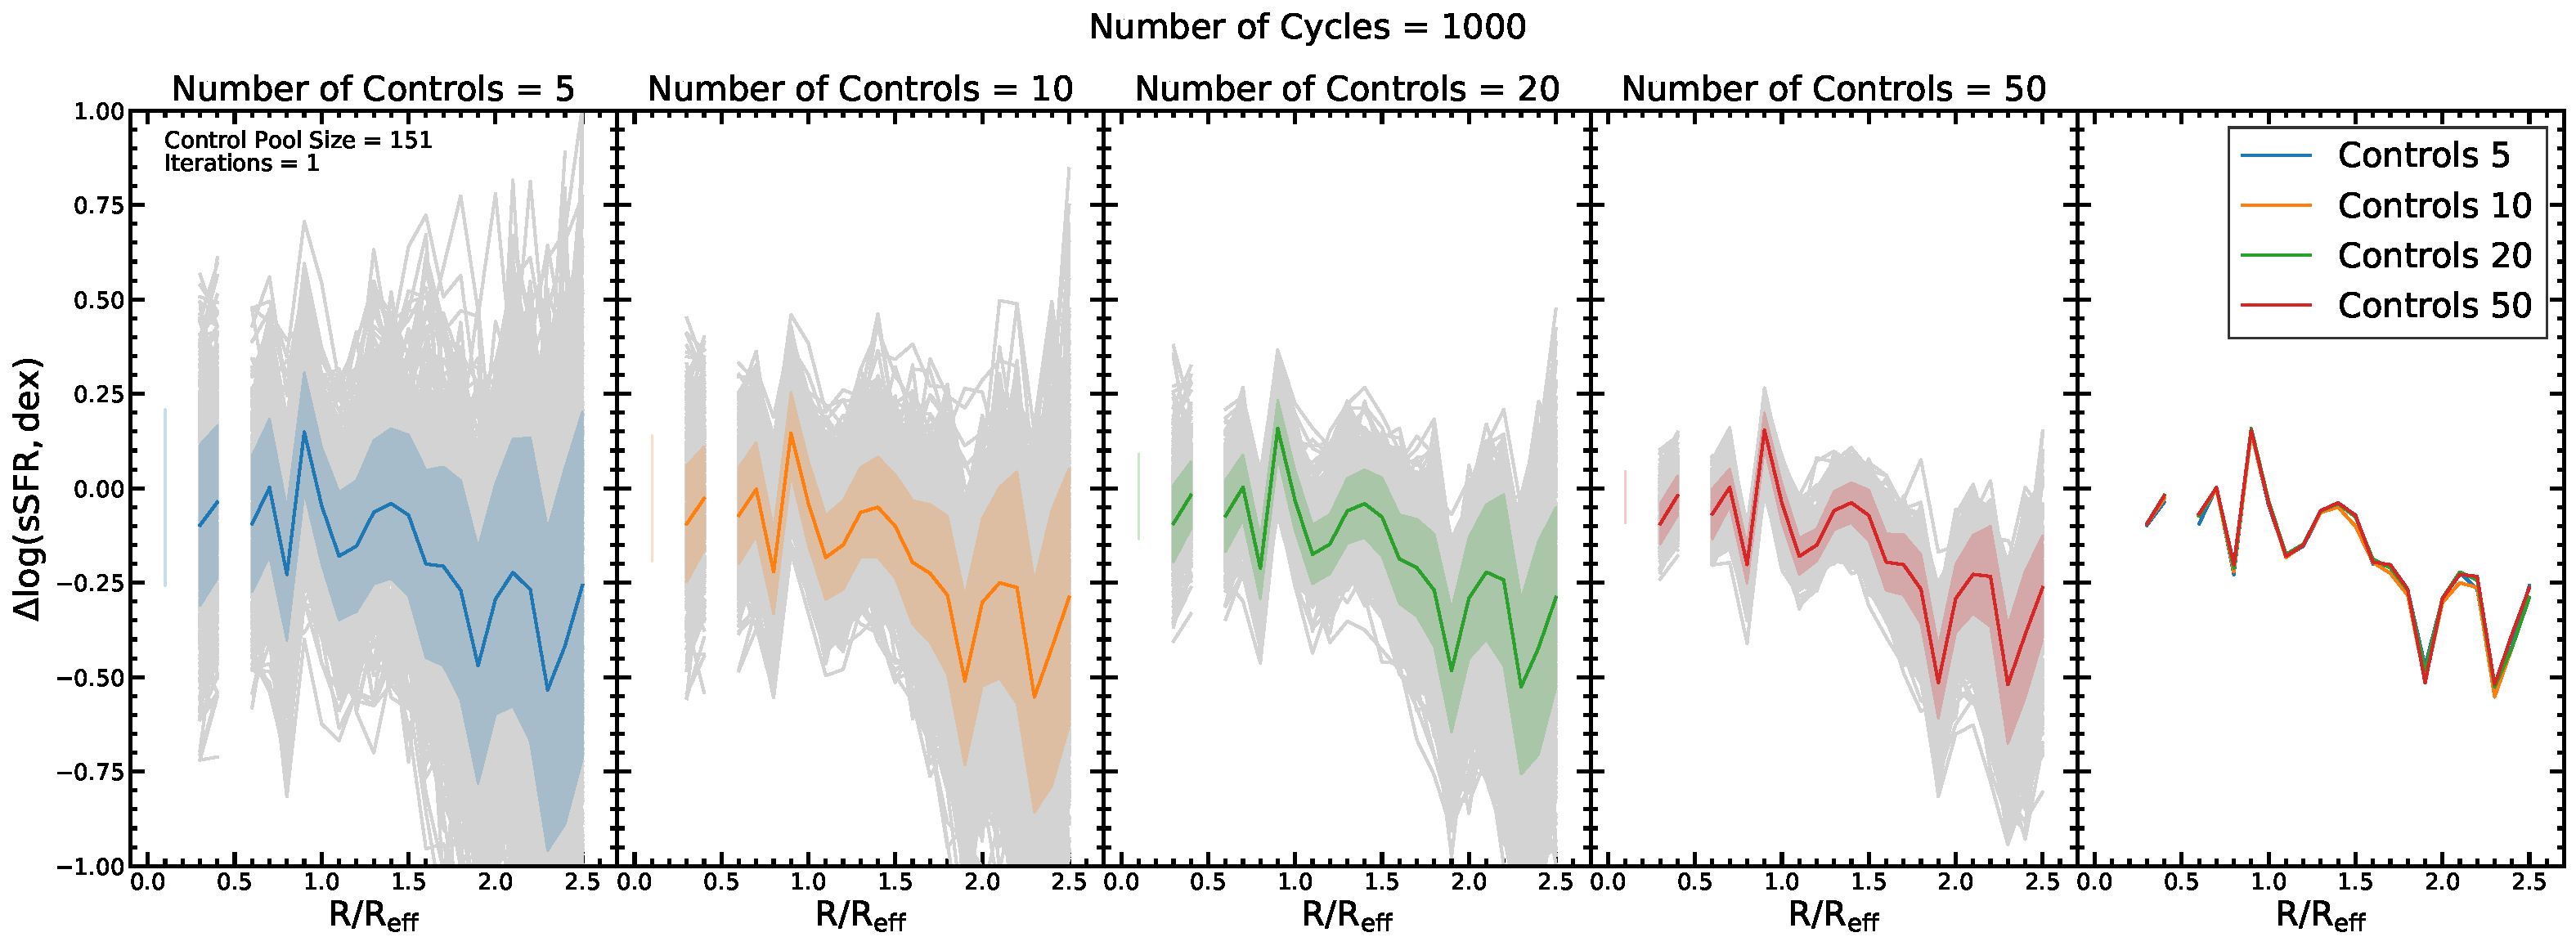
\includegraphics[width=\linewidth]{fig/8485-3704.pdf}
\caption[Example of bootstrapping to quantify the deviation of the random subsample of controls]{An example of the bootstrapping used to quantify the errors associated with the random selection of the control subsample. From left to right, the first four panels show the individual dex profiles after a random sub-selection in grey. The random sub-selection is run 1000 times and the median profile after the 1000 cycles is given by the colored profile. The highlighted region about the colored profiles is the standard error of the mean of the median profile. From left to right each panel shows the random selection for a different number of controls to select; 5, 10, 20, and 50 controls. The panel on the right end shows the median profiles of all of the preceding panels. }
\label{fig:bootstrap}
\end{figure*}
%%%%%%%%%%%%%%%%%%%%%%%%%%%%%%%%%%%%%%%%%%%%%%

%%%%%%%%%%%%%%%%%%%%%%%%%%%%%%%%%%%%%%%%%%%%%%
\begin{figure}
\centering
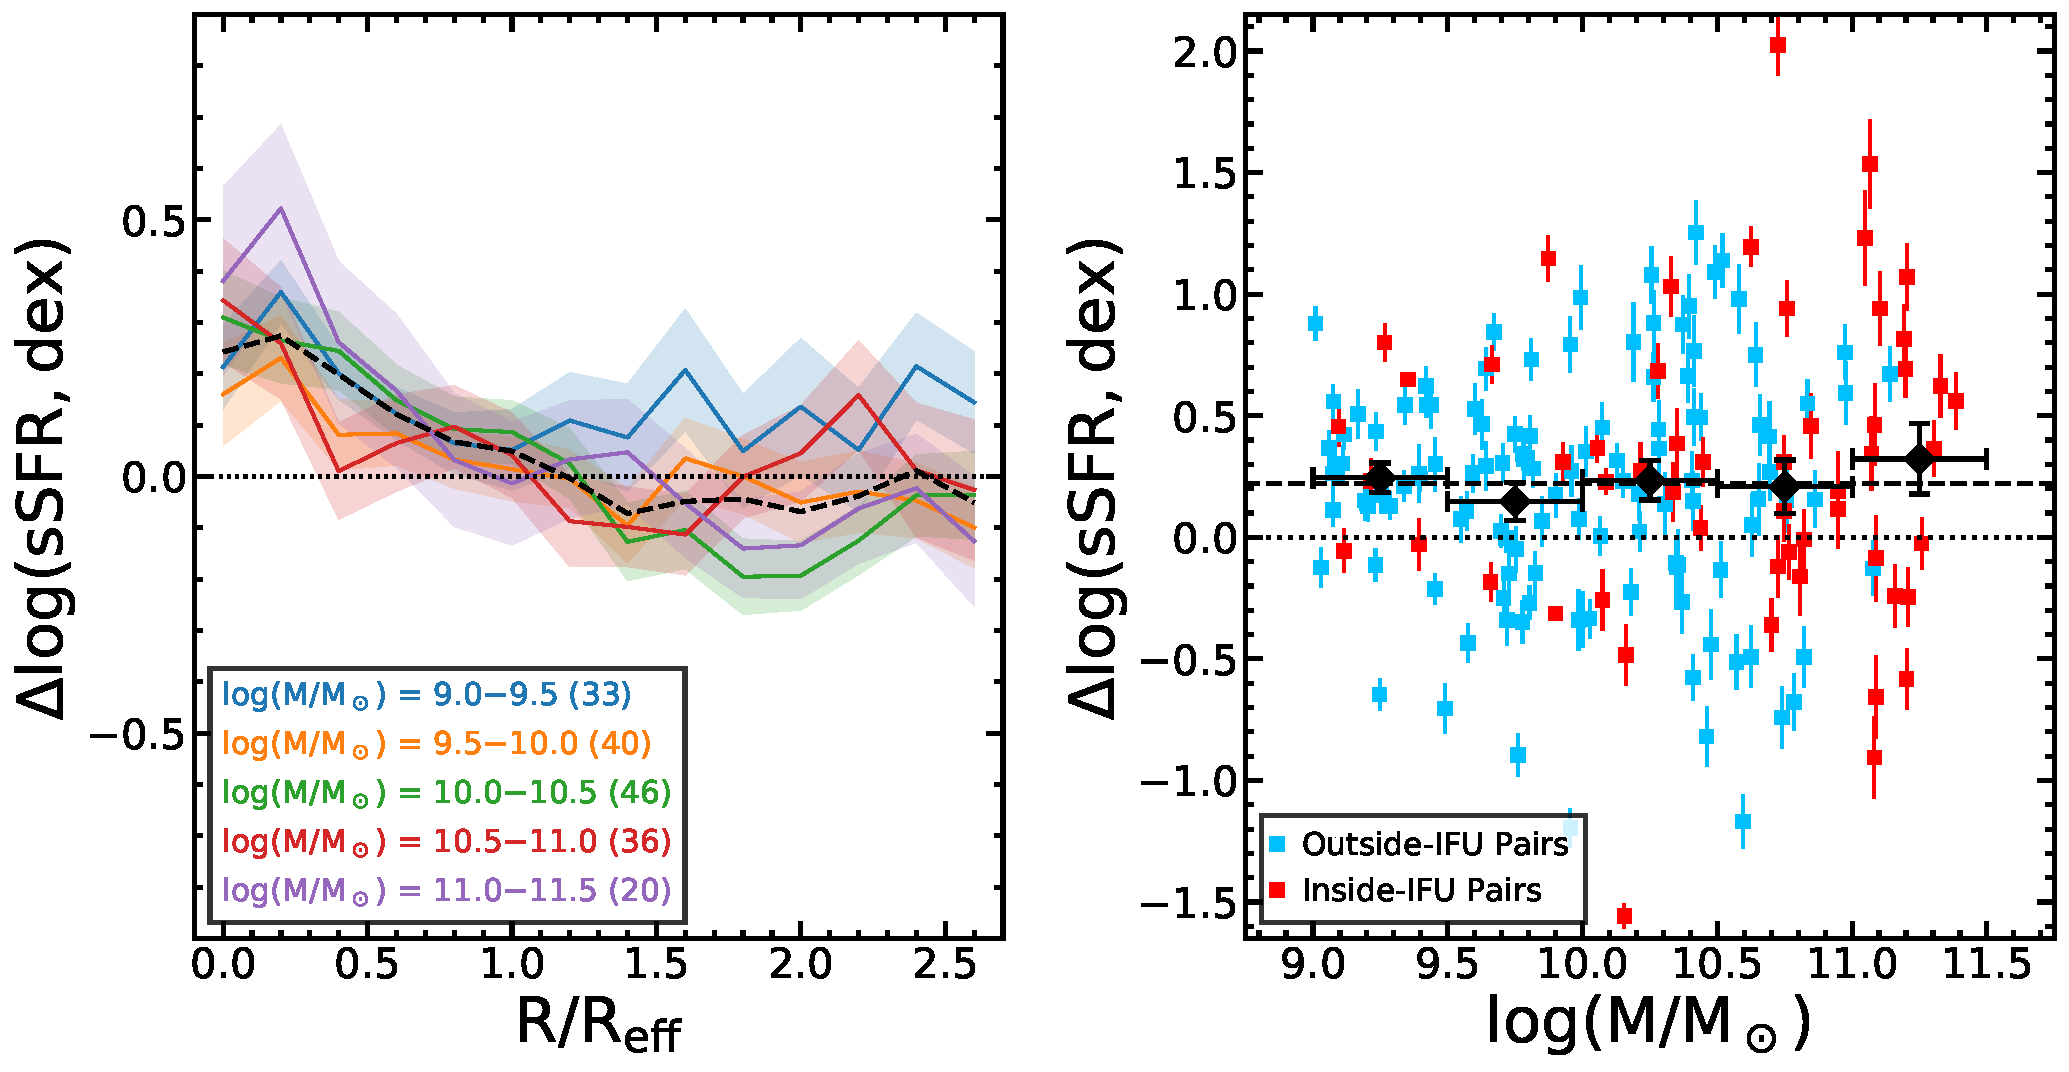
\includegraphics[width=\linewidth]{fig/ssfr_mass.pdf}
\caption[The $\Delta$log(sSFR) split by stellar mass.]{The $\Delta$log(sSFR) split into separate stellar mass bins. The left column gives the stacked difference profiles. The highlighted region about the profiles represents the standard error of the mean of the profile. The right column gives the nuclear $\Delta$log(sSFR) values. The black squares are the mean values within a stellar mass bin (where the size of the bins are shown the the horizontal error bars). The vertical error bars on the black squares represent the standard deviation within the bin. The top row is the inside-IFU sample, the middle row is the outside-IFU sample, and the bottom row is the combination of the two samples.}
\label{fig:ssfr_mass}
\end{figure}
%%%%%%%%%%%%%%%%%%%%%%%%%%%%%%%%%%%%%%%%%%%%%%

%%%%%%%%%%%%%%%%%%%%%%%%%%%%%%%%%%%%%%%%%%%%%%
\begin{figure}
\centering
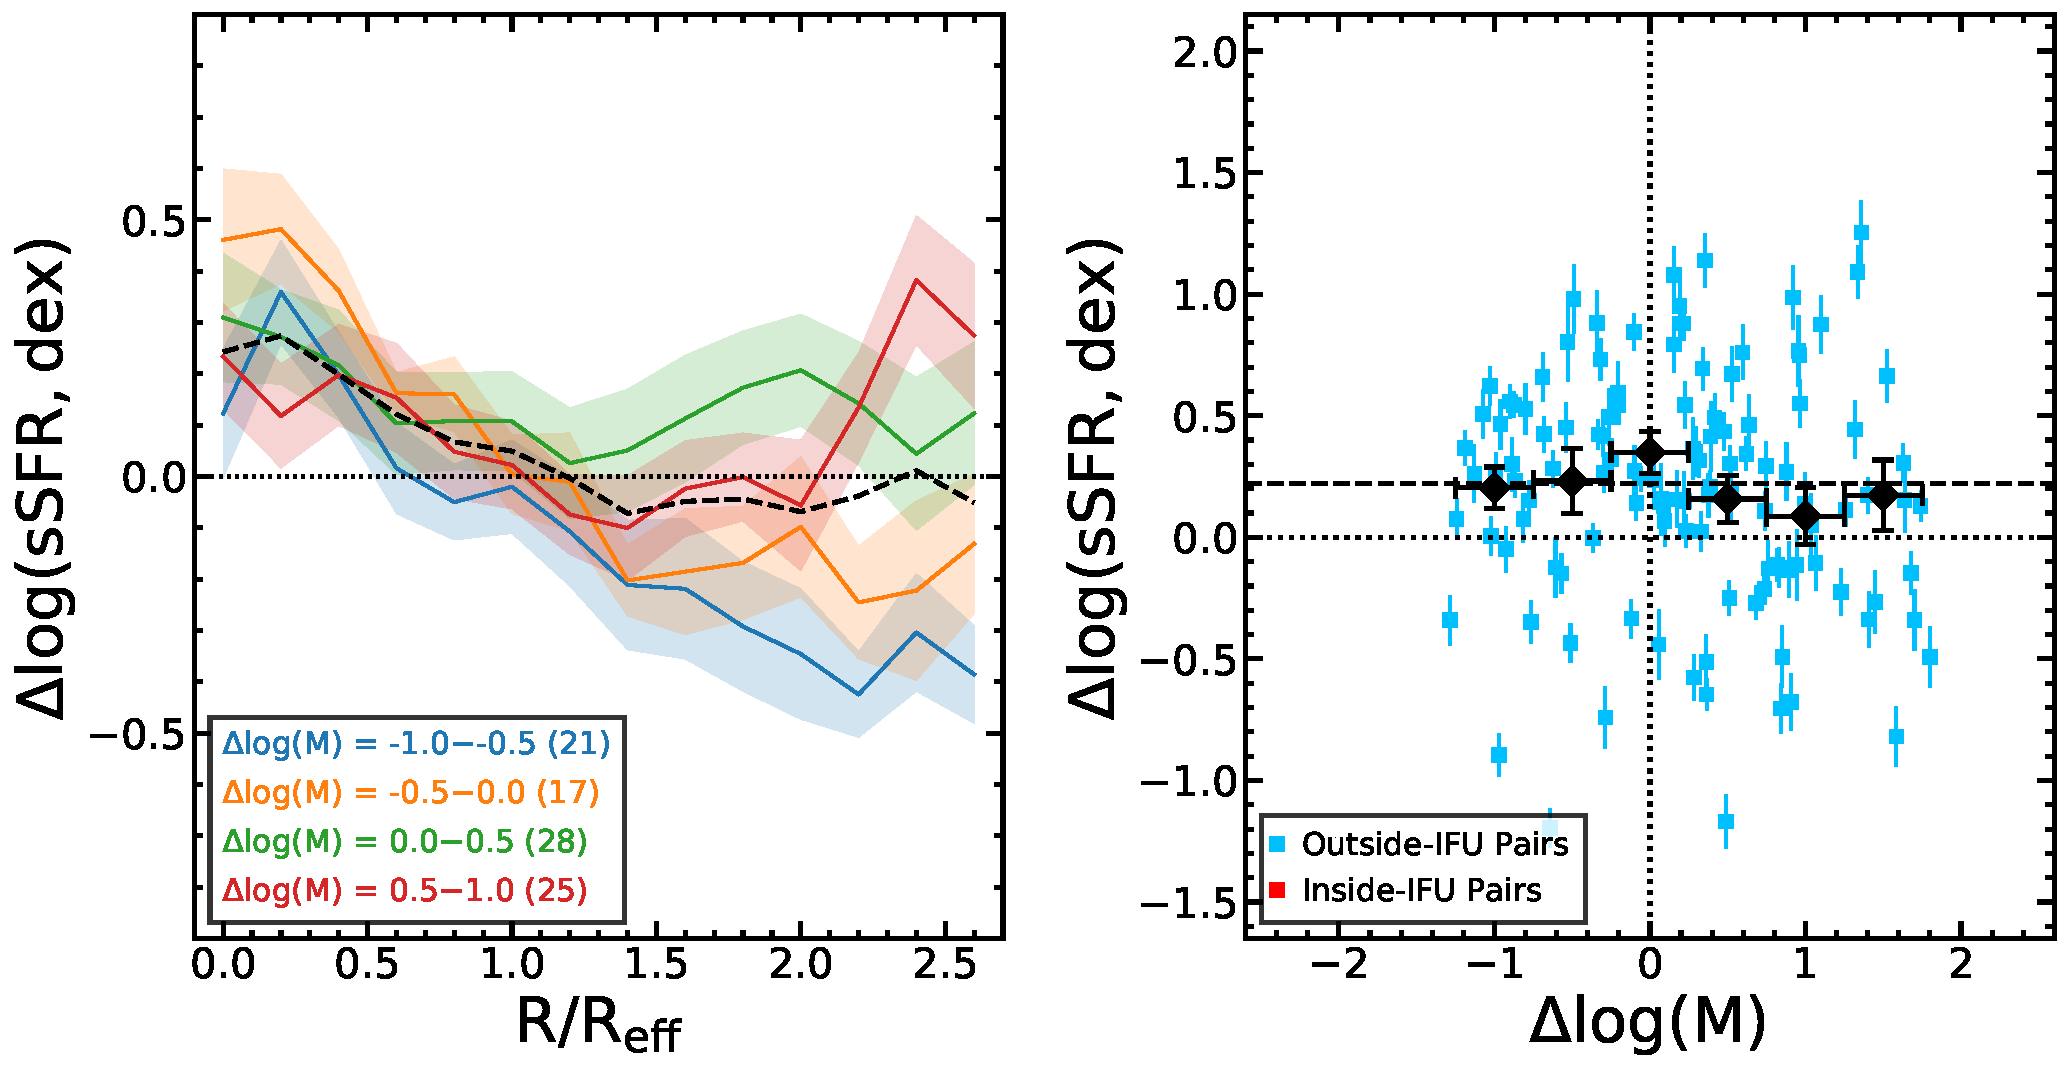
\includegraphics[width=\linewidth]{fig/ssfr_dm.pdf}
\caption[The $\Delta$log(sSFR) split by mass ratio.]{Same as Figure \ref{fig:ssfr_mass} but split into separate mass ratio bins.}
\label{fig:ssfr_dm}
\end{figure}
%%%%%%%%%%%%%%%%%%%%%%%%%%%%%%%%%%%%%%%%%%%%%%

%%%%%%%%%%%%%%%%%%%%%%%%%%%%%%%%%%%%%%%%%%%%%%
\begin{figure}
\centering
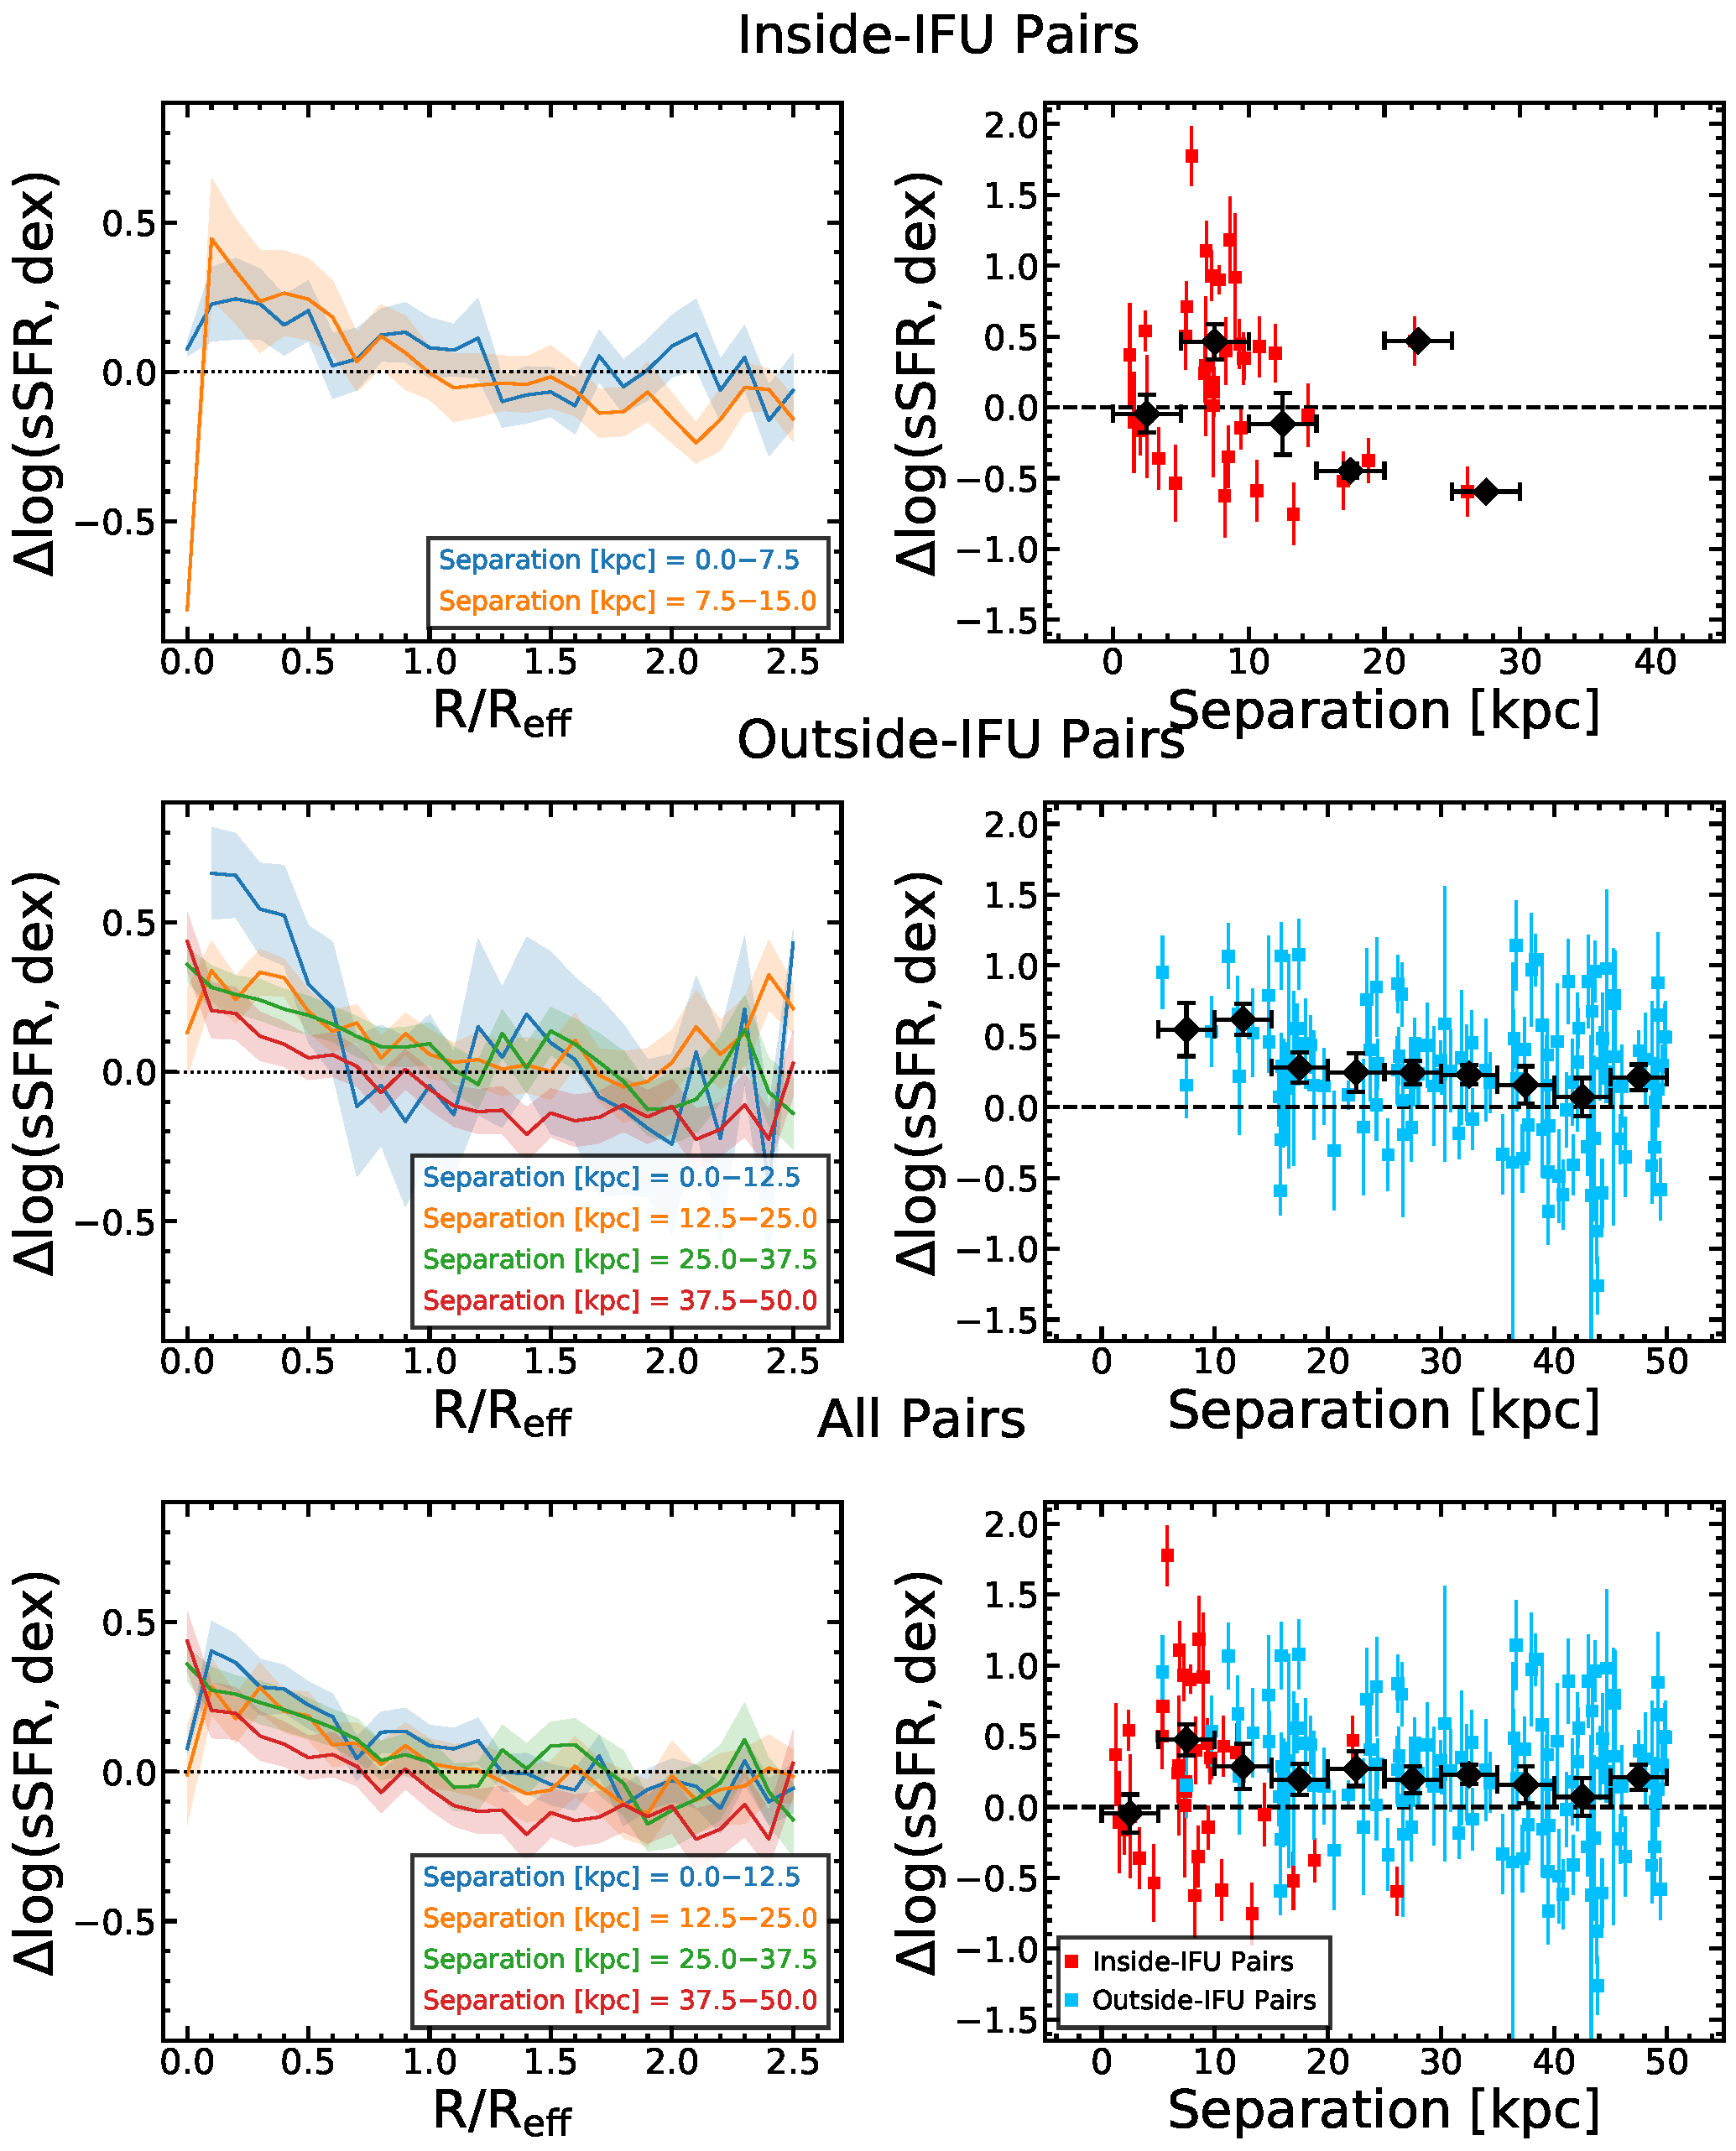
\includegraphics[width=\linewidth]{fig/ssfr_sep.pdf}
\caption[The $\Delta$log(sSFR) split by projected separation.]{Same as Figure \ref{fig:ssfr_mass} but split into separate projected separation bins.}
\label{fig:ssfr_sep}
\end{figure}
%%%%%%%%%%%%%%%%%%%%%%%%%%%%%%%%%%%%%%%%%%%%%%

%%%%%%%%%%%%%%%%%%%%%%%%%%%%%%%%%%%%%%%%%%%%%%
\begin{figure}
\centering
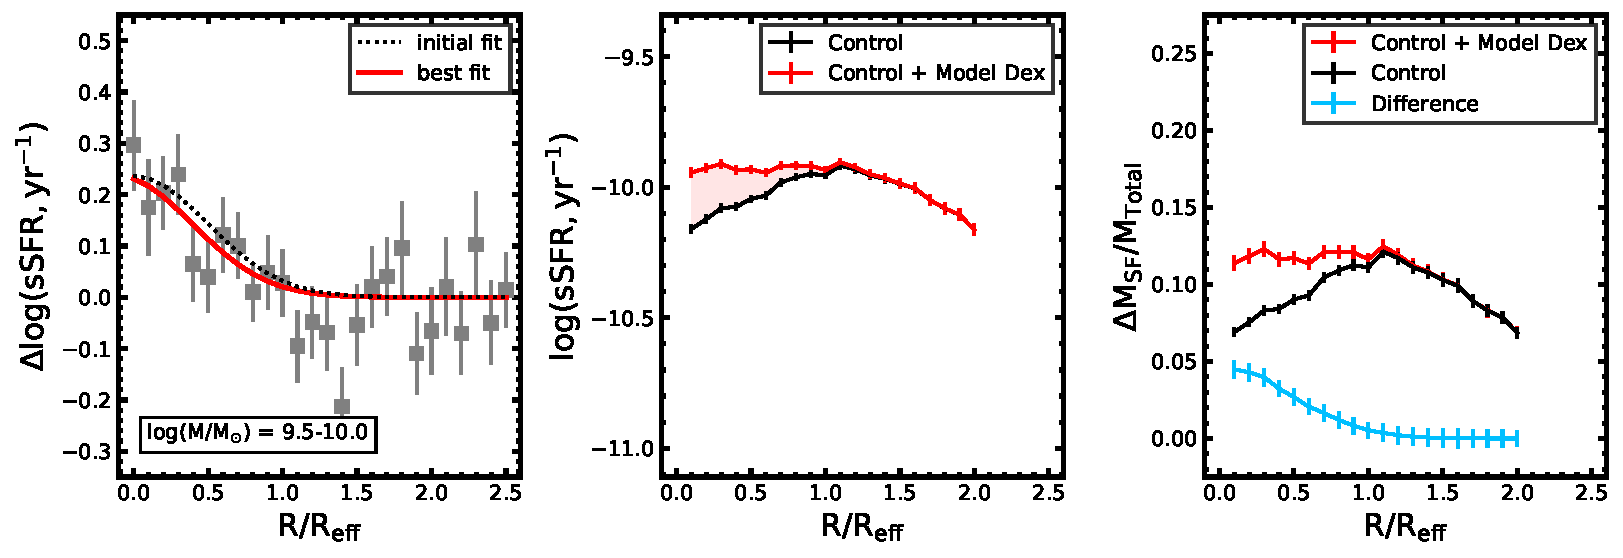
\includegraphics[width=\linewidth]{fig/mass_gain_1.pdf}
\caption[Example of the calculation of the fractional mass gain due to merger induced star formation for a single mass bin.]{In the Left panel we fit a model gaussian to the $\Delta$log(sSFR) profiles. In the Middle panel we plot the log(sSFR) profile for the stacked profiles of the control galaxies (black). We then add the modeled $\Delta$log(sSFR) profile to the control profile (red). The error bars represent the standard error of the mean of the profiles. In the Right panel we show the fractional mass gain due to star formation in the control galaxies (black) and in the paired galaxies (red). The blue profile is the subtraction between the pairs and controls and represents the fractional mass gain due to merger induced star formation. The error bars represent the standard error of the mean of the profiles. }
\label{fig:mass_gain}
\end{figure}
%%%%%%%%%%%%%%%%%%%%%%%%%%%%%%%%%%%%%%%%%%%%%%

%%%%%%%%%%%%%%%%%%%%%%%%%%%%%%%%%%%%%%%%%%%%%%
\begin{figure}
\centering
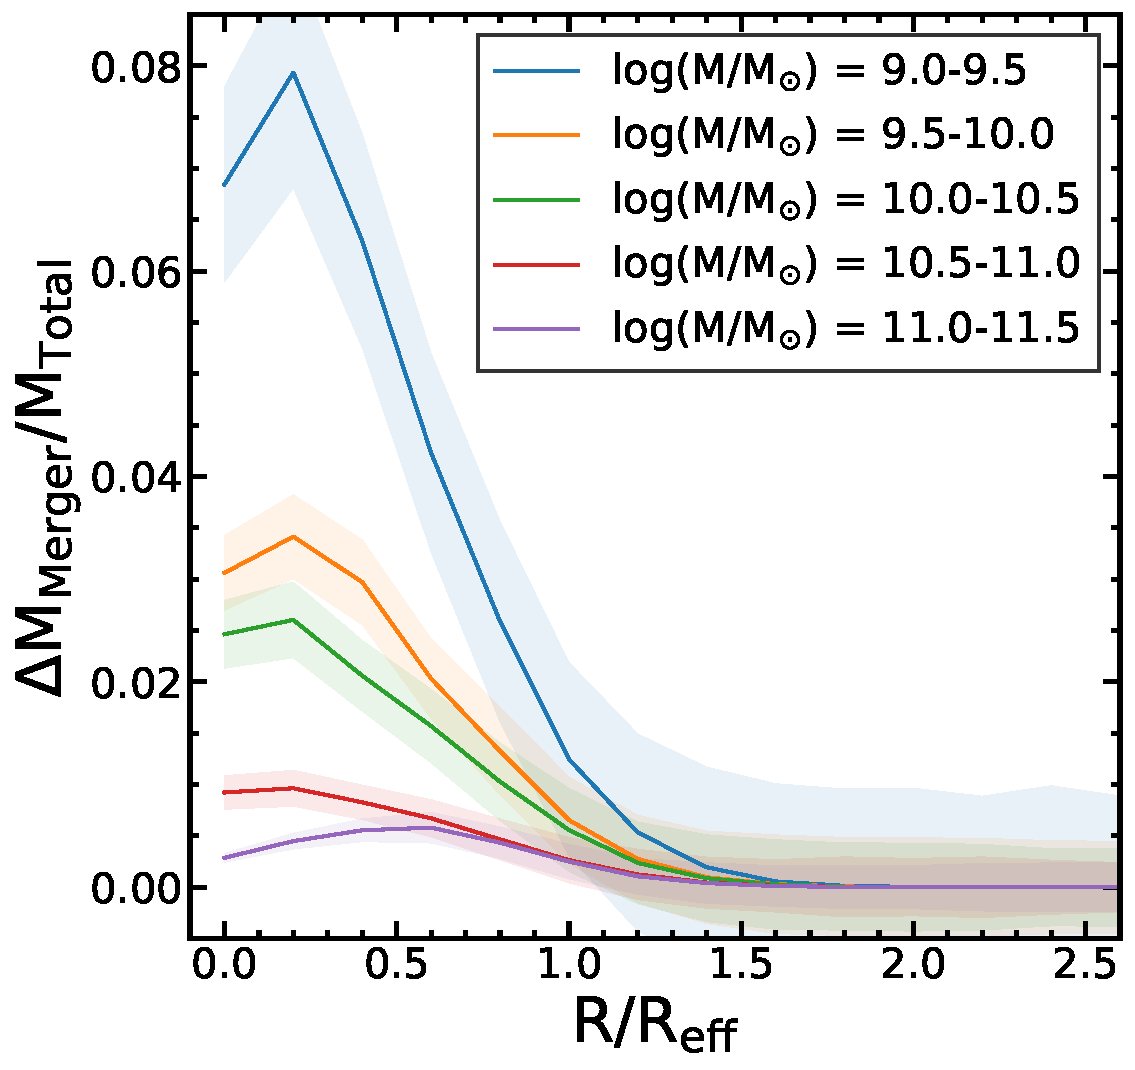
\includegraphics[width=3in]{fig/mass_gain.pdf}
\caption[The fractional mass gain due to merger induced star formation.]{The fractional mass gain due to merger induced star formation over a dynamical timescale, $\tau$ $=$ 1 Gyr. The highlighted region represents the propagated standard errors of the mean of the stacked log(sSFR) profiles. }
\label{fig:mass_gain_sum}
\end{figure}
%%%%%%%%%%%%%%%%%%%%%%%%%%%%%%%%%%%%%%%%%%%%%%

\end{document}